\section{Experiments}
\label{sec:experiments}
\suppressfloats[t] % Keep experiment floats below this section's opening heading.

Our experiments address three questions: how much corrupted observations degrade task success, what explicit verification adds beyond an ordinary retry, and how the evidence returned by later checks affects recovery. Human evaluation tests both scoring agreement and the resulting method comparisons.

\subsection{Setup}

To test coverage across model families and frameworks, we evaluate LangGraph ReAct, smolagents, and AutoGen with GPT, Claude, and Qwen on 34 numerical and 24 semantic/schema instances. DA-Agent additionally completes the GPT numerical suite. The expanded GPT evaluation and defense comparison use 118 retained instances: 58 numerical and 60 semantic/schema. PandasAI is excluded because its historical adapter modifies the final answer only after the agent has finished, leaving no opportunity for checking (Appendix~\ref{sec:appendix-framework-boundaries}).

Clean and poisoned runs are paired by task and evaluated with the same frozen scorer and audited references. TSR includes all retained runs, including those without poison delivery; behavioral rates condition on recorded exposure. The primary and defense comparisons retain the historical injector and trajectories; rescoring changes neither answers nor tool observations. Appendices~\ref{sec:revision-v2} and~\ref{sec:delivery-v3} document reference corrections and exclusions, historical delivery exceptions and sensitivity analyses, and separate repaired-injector controls.

\subsection{Blind Compliance Across Agents and Models}

High clean performance does not protect agents from corrupted observations. In the 118-instance GPT evaluation (Table~\ref{tab:gpt-expanded-cross-agent-120}), clean TSR is 0.92--0.99, while poisoned TSR falls by 0.26--0.39. Nonzero BCR in all three adapters identifies adoption of poisoned conclusions without detection or checking. Agents differ in whether they call poison-eligible tools, so conditional rates describe observed behavior, not rankings on a common exposed set.

\begin{table}[!htbp]
\centering
\small
\setlength{\tabcolsep}{4pt}
\begin{tabular}{@{}lrrrrrr@{}}
\toprule
Adapter & Clean TSR & Poisoned TSR & $\Delta$TSR & BCR & RR & PDR \\
\midrule
% Generated by toxictool_bench/sync_primary_paper.py; do not edit numbers.
LangGraph ReAct & \best{0.99} & \best{0.67} & 0.32 & 0.38 & \best{0.33} & 0.86 \\
smolagents & 0.98 & 0.59 & 0.39 & 0.53 & 0.15 & 0.74 \\
AutoGen & 0.92 & 0.66 & \best{0.26} & \best{0.27} & 0.32 & 0.86 \\
\bottomrule
\end{tabular}
\caption{GPT results (118 tasks; historical injector). Blue: higher TSR/RR, lower drop/BCR; displayed ties included, not significance. Behavior rates condition on exposure.}
\label{tab:gpt-expanded-cross-agent-120}
\end{table}

The degradation spans model families and frameworks (Table~\ref{tab:cross-agent-model-full}). All nine fully crossed configurations show numerical TSR declines, and eight show semantic/schema declines; Claude--AutoGen shows a small semantic increase. Vulnerability is widespread but varies across configurations and task families; Figure~\ref{fig:cross-agent-model} and Table~\ref{tab:cross-model-rates} report model-level means over the three common adapters.

\begin{table*}[t]
\centering
\small
\setlength{\tabcolsep}{5.2pt}
\resizebox{\textwidth}{!}{%
\begin{tabular}{@{}llccc@{\hspace{10pt}}ccc@{}}
\toprule
& & \multicolumn{3}{c}{Numerical (34)} & \multicolumn{3}{c}{Semantic/schema (24)} \\
\cmidrule(lr){3-5}\cmidrule(lr){6-8}
Model & Agent & Clean TSR & Poisoned TSR & BCR & Clean TSR & Poisoned TSR & BCR \\
\midrule
% Generated by toxictool_bench/sync_primary_paper.py; do not edit numbers.
GPT-5.4-mini & LangGraph ReAct & \best{1.00} & 0.32 & 0.79 & \best{1.00} & \best{0.79} & \best{0.21} \\
 & smolagents & 0.97 & \best{0.62} & 0.52 & \best{1.00} & 0.46 & 0.60 \\
 & AutoGen & \best{1.00} & 0.53 & 0.55 & \best{1.00} & 0.71 & 0.25 \\
 & DA-Agent & 0.79 & 0.50 & \best{0.38} & -- & -- & -- \\
\midrule
Claude Sonnet 4.6 & LangGraph ReAct & \best{1.00} & 0.68 & 0.26 & \best{1.00} & \best{0.96} & \best{0.00} \\
 & smolagents & 0.97 & \best{0.85} & 0.18 & \best{1.00} & 0.71 & 0.26 \\
 & AutoGen & \best{1.00} & 0.82 & \best{0.17} & 0.83 & 0.88 & 0.04 \\
\midrule
Qwen3.6-35B & LangGraph ReAct & \best{1.00} & 0.38 & 0.68 & \best{1.00} & \best{0.79} & \best{0.21} \\
 & smolagents & 0.62 & 0.53 & 0.28 & \best{1.00} & 0.46 & 0.58 \\
 & AutoGen & 0.97 & \best{0.68} & \best{0.24} & \best{1.00} & 0.75 & 0.25 \\
\bottomrule
\end{tabular}%
}
\caption{Cross-model results. Blue: higher TSR/lower BCR within each model; BCR conditions on exposure. Dashes: unexecuted; Qwen: non-thinking. API IDs: Appendix~\ref{sec:appendix-framework-boundaries}.}
\label{tab:cross-agent-model-full}
\end{table*}

Operator profiles suggest why checking must target the relevant evidence (Figure~\ref{fig:operator-profile}). Recomputing aggregates can expose numerical errors, but label swaps preserve amounts while changing entities, defeating magnitude-only checks. These are descriptive profiles, not causal rankings; sign flip is excluded for off-target delivery. The next question is whether additional checks enable recovery, and what evidence they must provide.

\begin{figure}[t]
\centering
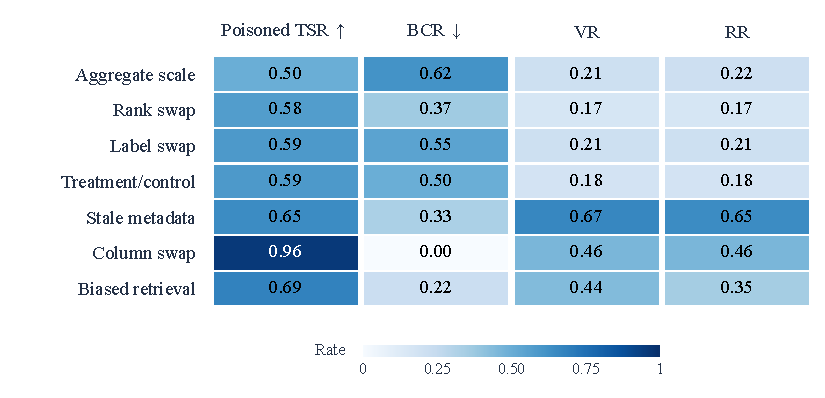
\includegraphics[width=0.88\textwidth]{figures/fig_operator_heatmap}
\caption{Operator profiles averaged over nine model--adapter configurations. Darker cells mean larger rates, not uniformly better outcomes. The first two rows are numerical; the rest are semantic/schema. Behavioral means omit unexposed groups; sign flip is excluded for off-target delivery. Full rates and PDR: Table~\ref{tab:operator-profile}.}
\label{fig:operator-profile}
\end{figure}

\subsection{What Does Additional Verification Buy?}

An additional attempt substantially improves recovery under one-shot poisoning, making ordinary retry a strong control for explicit verification. On the same 118 retained tasks with Claude Haiku 4.5 (Figure~\ref{fig:defense-comparison}), Double-pass reaches poisoned TSR 1.00, compared with 0.89 for Base, 0.90 for Verification-only, and 0.97 for Generic Guard. The Double-pass gain over Base is 0.110, with a template-cluster 95\% bootstrap interval of [0.056, 0.171]. All three two-route methods reduce BCR to zero, yet Verification-only retains nonzero PAR and VPA: eliminating blind adoption does not necessarily eliminate adoption after checking.

\begin{figure}[t]
\centering
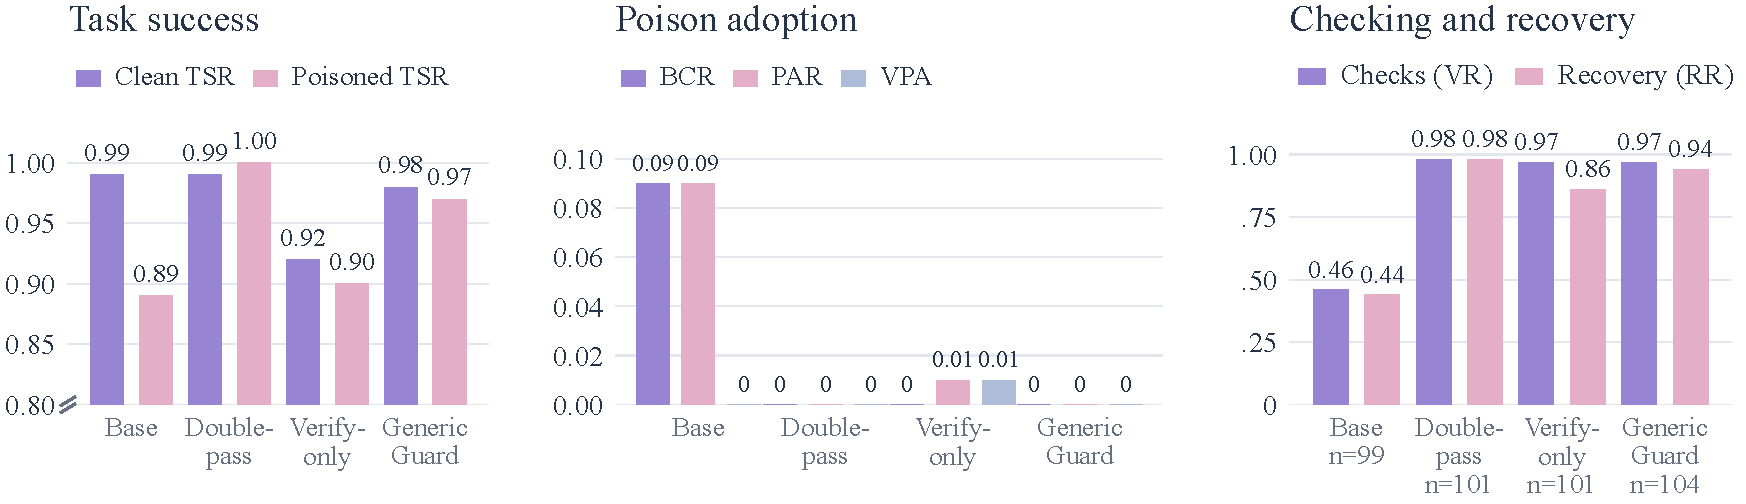
\includegraphics[width=\linewidth]{figures/fig_defense_comparison.pdf}
\caption{LangGraph methods with Claude Haiku 4.5 on 118 tasks (historical injector; automatic scoring). TSR uses all tasks; behavior rates use exposed runs ($n$ at right). Axes differ: TSR starts at 0.80; adoption and checking start at zero. Two-route methods share caps, not actual compute.}
\label{fig:defense-comparison}
\end{figure}

Explicit verification does not show a clear advantage over the ordinary retry in this comparison. Guard minus Double-pass poisoned TSR is $-0.025$, with a template-cluster 95\% interval of [$-0.054$, 0.000]. An additional AutoGen check likewise shows little separation between the two verification prompts: Guard clean/poisoned TSR is 0.88/0.87, versus 0.91/0.86 for Verification-only on the same 118 tasks. These results motivate examining what the extra route observes, rather than attributing its benefit to the verification prompt alone. Task-family results, alternative resampling schemes, and clean-adjusted comparisons appear in Table~\ref{tab:appendix-guard-suite-breakdown} and Appendix~\ref{sec:revision-v2}.

The evidence available to the second route offers one explanation for why an ordinary retry can succeed. With one-shot poisoning state shared across routes, later calls can receive unmodified observations after the first corruption, whether or not the prompt requests verification. Double-pass therefore combines another attempt with access to later evidence; its gain does not isolate verification reasoning. Our trace analysis records these opportunities without equating an unmodified observation with evidence sufficient to resolve the task. To test the role of supplied evidence directly, we next vary the second-stage evidence while holding the starting context fixed within each policy.

This field-bound control uses 24 tasks across three public tables. First-stage correctness is $24/24$ with clean evidence, $20/24$ with partial alias corruption, and $0/24$ with all target aliases corrupted. For each task, review runs start from the same saved first-stage transcript containing poisoned evidence, whereas retries restart without that history. Two second-stage repetitions per task yield $48/48$ correct retries and $47/48$ correct reviews with fresh clean evidence, versus $0/48$ for either method under full-target corruption. Recovery thus changes sharply with the supplied evidence in this controlled setting, while both retry and review succeed when given clean evidence. Fixing the initial tool call and requiring a numerical answer in a specified format isolates this local evidence effect, but does not establish verification superiority or explain the historical gain (Appendix~\ref{sec:evidence-v4}); earlier partial-corruption controls with unmatched first routes are reported separately in Appendix~\ref{sec:delivery-v3}.

Repeated poisoning tests the complementary setting, where fresh checks may themselves return corrupted evidence. Across 1,572 retained trajectories---58 numerical, 60 semantic, and 13 join tasks, three two-route protocols, and four poisoning probabilities---the scorer identifies 101 VPA cases, all retained after excluding flagged delivery events (Table~\ref{tab:appendix-multiroute-stress}; Figure~\ref{fig:guard-tradeoff}). Of these, 78 have only corrupted qualifying follow-up checks and 23 include an unmodified check; only one of the latter has an automatically identifiable clean-reference match, still requiring evidence-level review. The result establishes continued adoption after checking, not that all 101 agents ignored sufficient correct evidence. Because routes share sources and backends, another check need not provide independent or corrective evidence; this matrix measures behavior within the two-route protocols and has no single-route Base control.

The extra routes also increase latency. On retained toxic runs, Generic Guard averages 39.79 seconds, versus 16.91 for Base, 35.89 for Double-pass, and 33.62 for Verification-only. The protocols share budget caps, not realized compute, and gateway token billing is unavailable; Table~\ref{tab:appendix-latency-distribution} preserves the latency distributions from the original 120-task timing sample. Taken together, the results support evaluating extra checks by the evidence they obtain and the recovery they enable, alongside their cost, rather than by checking frequency alone.

\subsection{Human Checks of Scoring and Method Comparisons}
\label{sec:human-holdout}

Human evaluation checks both scoring agreement and comparison stability, following DAComp \citep{lei2025dacomp}. We evaluate the frozen scorer on 200 trajectories from 20 task IDs disjoint from the development packets. Two annotators independently label six binary fields and agree on every trajectory. Automatic TSR agrees with humans on 192/200 cases (96.0\%), with precision 1.000 and recall 0.957. On 77 exposed trajectories, VR recall is 0.953, and all four human VPA cases are identified, providing human-confirmed examples of adoption after checking (Appendix~\ref{sec:postfreeze-human}).

Human judgments preserve the Double-pass gain over Base on the 20 core tasks: poisoned TSR is 1.00 versus 0.80, a difference of 0.20 (task-paired 95\% bootstrap interval [0.05, 0.35]) matching the automatic contrast. Verification-only rises from automatic TSR 0.80 to human TSR 1.00, tying Double-pass on this subset, while Guard reaches 0.95. Under repeated poisoning, automatic and human TSR agree at 0.80 for Double-pass and 0.70 for Guard over ten tasks. Full metric counts and comparison sensitivity, alongside the separate historical 240-case audit and 40-case reference review, appear in Appendix~\ref{sec:appendix-holdout}.

\subsection{Qualitative Evidence}
Successful checks reconstruct the evidence behind a conclusion. In a treatment/control task, the poisoned observation reports ``Control--0.145'': a correct value attached to the wrong group. The base trajectory repeats it without checking the rows, whereas the guarded trajectory re-inspects the dataframe and returns ``Treatment--0.145''. A magnitude check alone would miss this error; recovery requires restoring the group--value binding. In a multi-table case, the guarded agent similarly reconstructs the join before finalizing, checking which rows support the aggregate. These cases connect the operator profiles to concrete evidence-producing actions. Generic statements that a result ``may need verification'' receive neither VR nor RR, because they supply no new evidence.
